\chapter{Sigilo Perfeito}
\label{cha:sigilo-perfeito}

No final dos anos 40, com o desenvolvimento dos primeiros computadores e a experiência da quebra das cifras mecanicamente produzidas por poderosas máquinas desenvolvidas pelo esforço de guerra do nazismo, alguns cientístas se voltaram para um problema central no campo da criptografia: o que torna um sistema de criptografia seguro?
As cifras que vimos até agora são conhecidas como ``cifras clássicas'' exatamente porque elas precedem desse debate moderno, e não a toa foram todas derrotadas cedo ou tarde.
Informalmente, poderíamos dizer que o problema dos esquemas clássicos de criptografia é que eles guardam muita informação sobre a mensagem (frequência das letras, dos dígrafos, letras duplas etc.). 
Não é uma coincidência, portanto, que a primeira tentativa de formalizar o conceito de segurança tenha sido proposto por Claude Shannon, o fundador da teoria da informação.
Shannon definiu o que hoje chamamos de {\em sigilo perfeito}.
Um esquema de criptografia garante o sigilo perfeito se a cifra não guarda nenhuma informação sobre a mensagem que a gerou.
Ou, de maneira um pouco mais descritiva, se a probabilidade da cifra ocorrer é independente da probabilidade da mensagem:

\begin{definition}
  Um esquema de criptografia simétrica $\Pi = \langle Gen, E, D \rangle$ garante o {\em sigilo perfeito} se, supondo que $Pr[C=c] > 0$, para toda distribuição de probabilidade sobre $M$ temos que:
\begin{displaymath}
  Pr[M = m | C = c] = Pr[M = m]
\end{displaymath}

Ou de maneira equivalente se para todo $m_0, m_1 \in M$ e todo $c \in C$ temos que:
\begin{displaymath}
  Pr[C = c | M = m_0] = Pr[C = c | M = m_1]
\end{displaymath}
\end{definition}

Essa segunda formulação é mais intuitiva, ela estabelece que um sistema garante o sigilo perfeito se a probabilidade de $m_0$ produzir a cifra $c$ é idêntica a probabilidade de qualquer outra mensagem $m_1$ produzir a mesma cifra $c$.
O exemplo a seguir mostra que a cifra de substituição não garante o sigilo perfeito:

\begin{example}
  Seja $\Pi = \langle Gen, E, D \rangle$ o sistema de criptografia de substituição e sejam $c = \textrm{\tt ANA}$, $m_0 = \textrm{\tt OVO}$ e $m_1 = \textrm{\tt EVA}$.
Como o sistema $\Pi$ substitui cada letra da mensagem por uma letra na cifra, existem chaves $k$ tal que $E(k, m_0) = c$ -- basta que $k(\textrm{\tt O}) = \textrm{\tt A}$ e $k(\textrm{\tt V}) = \textrm{\tt N}$, de fato a chance de escolher uma chave assim é $\frac{1}{26 \cdot 25} = \frac{1}{650}$ --, mas não existe nenhuma chave $k'$ tal que $E(k', m_1) = c$.
Portanto temos que:
\begin{displaymath}
Pr[C = c | M = m_0] =  \frac{1}{650} \neq Pr[C = c | M = m_1] = 0  
\end{displaymath}
\end{example}

Uma forma equivalente, e útil como veremos mais para frente, de definir sigilo perfeito é a partir de um jogo.
Imaginamos que há um adversário $\mathcal{A}$ cujo objetivo é quebrar a cifra produzida pelo sistema $\Pi$.
O jogo funciona da seguinte maneira: 
\begin{enumerate}
\item $\mathcal{A}$ escolhe duas mensagens $m_0$ e $m_1$ com o mesmo tamanho ($|m_0| = |m_1|$) e envia para o sistema $\Pi$.
\item O sistema gera uma chave $k$ usando o algoritmo $Gen$ e sorteia aleatoriamente uma das mensagens para criptografar ($\Pi$ sorteia $b \leftarrow \{0, 1\}$ e criptografa $m_b$).
\item A cifra produzida $E(k, m_b) = c$ é enviada de volta para o adversário.
\item O adversário $\mathcal{A}$ produz um bit $b' \in \{0,1\}$.
\end{enumerate}

O desafio do adversário é acertar qual das duas mensagens foi cifrada.
O diagrama abaixo ilustra o processo:

\begin{center}
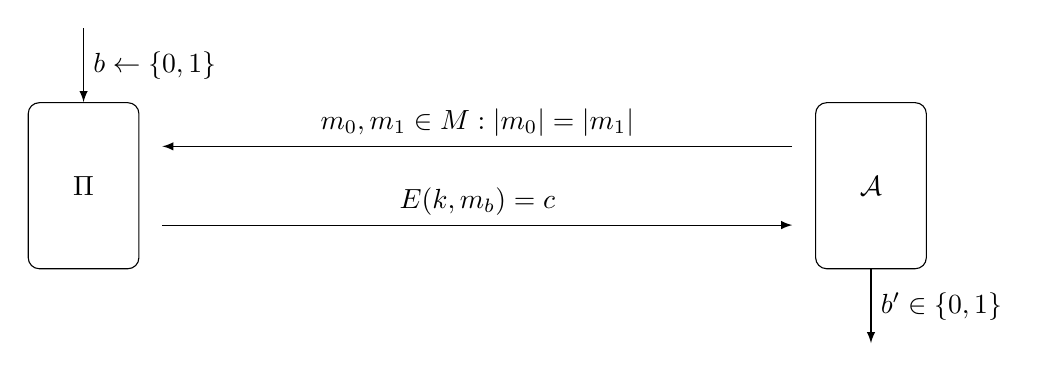
\begin{tikzpicture}[node distance=2cm,auto,>=latex]
\tikzset{
  player/.style={draw,shape=rectangle,rounded corners,minimum width=4em,minimum height=6em}
}
\node[player] (system) {$\Pi$};
\node[player] (adversary) at (10,0) {$\mathcal{A}$};
\draw[->] (9,.5) -> node[above]{$m_0, m_1 \in M : |m_0| = |m_1|$} (1,.5);
\draw[->] (1,-.5) -> node[above]{$E(k,m_b) = c$} (9,-.5);
\draw[->] (0,2) -> node{$b \leftarrow \{0,1\}$} (system);
\draw[->] (adversary) -> node{$b' \in \{0,1\}$} (10,-2);
\end{tikzpicture}
\end{center}

Chamamos o experimento ilustrado pelo diagrama de $PrivK^{eav}_{\Pi, \mathcal{A}}$.
Os subscritos indicam que o experimento depende do sistema $\Pi$ e do adversário $\mathcal{A}$.
O resultado do experimento deve ser $0$ se o adversário perdeu o desafio e $1$ caso contrário.
Formalmente temos que:
\begin{displaymath}
  PrivK^{eav}_{\Pi, \mathcal{A}} = \left\{
    \begin{array}{lcl}
      1 & \textrm{se} & b = b'\\
      0 & \textrm{c.c.} &\\
    \end{array}
    \right.
\end{displaymath}

É possível provar que um sistema $\Pi$ garante o {\em sigilo perfeito} se e somente se para qualquer adversário $\mathcal{A}$ temos que:
\begin{displaymath}
Pr[PrivK^{eav}_{\Pi, \mathcal{A}} = 1] = \frac{1}{2}
\end{displaymath}

Em palavras, o sistema possui sigilo perfeito se nenhum adversário é capaz de acertar qual das mensagens produziu a cifra $c$ com probabilidade melhor do que um meio.

\section{One Time Pad}
\label{sec:otp}

Temos agora uma definição formal de segurança.
Vimos que a cifra de substituição não satisfaz essa definição, mas na verdade nenhuma das cifras clássicas a satisfaz.
Não seria desejável que essas cifras satisfizessem a definição, pois vimos no capítulo anterior que nenhuma das cifras clássicas é segura e todas podem ser derrotadas se o adversário tiver acesso a uma cifra de tamanho suficientemente grande.
Ficamos então com o desafio de encontrar algum sistema que satisfaça essa definição, caso tal sistema exista.

No que segue, apresentaremos um sistema chamado {\em One Time Pad} (OTP), também conhecido como {\em cifra de Vernan}, e mostraremos que ele garante o sigilo perfeito.
A partir deste ponto, conforme começarmos a investigar sistemas a serem implementados computacionalmente, consideraremos que o espaço $M$ das mensagens (assim como o espaço $C$ das cifras) será representado como sequências de bits.
No caso específico do OTP assumiremos que as mensagens e a cifras possuem um tamanho fixo $n$.
Mais importante é o fato de que o universo das chaves é também um conjunto de sequências de bits do mesmo tamanho.
Assim temos que $M = C = K = \{0,1\}^n$.
O sistema $\Pi = \langle Gen, E, D \rangle$ é definido pelos seguintes algoritmos:
\begin{itemize}
\item $Gen := k \leftarrow \{0,1\}^n$
\item $E(k,m) = [m_0 + k_0\ mod\ 2] \dots [m_n + k_n\ mod\ 2] = m \xor k$
\item $D(k,c) = [c_0 + k_0\ mod\ 2] \dots [c_n + k_n\ mod\ 2] = c \xor k$
\end{itemize}

Para verificar a corretude do sistema basta notar que:

\begin{eqnarray*}
  D(k, E(k, m)) & = & D(k, k \xor m)\\
                & = & k \xor (k \xor m)\\
                & = & (k \xor k) \xor m\\
                & = & m
\end{eqnarray*}

A derivação usa o fato de que a operação de {\em ou exclusivo} $\xor$ é associativa, que $x \xor x = 1$ e $1 \xor x = x$ para todo sequência de bits $x \in \{0,1\}^*$.
Deixamos como exercício mostrar essas três propriedades da operação.

\begin{example}
  Considere uma mensagem $m = 101010$ e uma chave $k = 010001$.
Usando o sistema One Time Pad a cifra produzida é a seguite:

\begin{displaymath}
  \begin{array}{ccccc}
    m & \xor & k & = & c \\
    101010 & \xor & 010001 & = & 111011
  \end{array}
\end{displaymath}
\end{example}

Como antecipado, é possível, e relativamente simples provar que o OTP possui sigilo perfeito.

\begin{theorem}
  O sistema de criptografia {\em One Time Pad} possui sigilo perfeito.
\end{theorem}

\begin{proof}
  Seja $K = M = C = \{0,1\}^n$.
  Dada uma cifra $c \in C$ e uma mensagem qualquer $m \in M$, existe uma única chave $k \in K$ tal que $E(k,m) = c$.
  A chave é exatamente $k = m \xor c$, pois:
  
  \begin{eqnarray*}
    E(k, m) & = & k \xor m \\
            & = & (m \xor c) \xor m\\
            & = & (m \xor m) \xor c\\
            & = & c
  \end{eqnarray*}

Como existe exatamente uma chave possível que faz com que $E(k,m) = c$, temos que a probabilidade de se produzir $c$ dado uma mensagem qualquer $m$ é igual a probabilidade de sortear uma chave específica no universo $K = \{0,1\}^n$ que é $\frac{1}{2^n}$:
\begin{displaymath}
  Pr[C = c | M = c] = \frac{1}{2^n}
\end{displaymath}

Essa probabilidade é idêntica para qualquer $m \in M$.
Portanto, temos que $Pr[C = c| M = m_0] = Pr[C = c | M = m_1] = \frac{1}{2^n}$. 
\end{proof}

O {\em One Time Pad} possui duas severas limitações.
A primeira é indicada pelo próprio nome do sistema.
O sistema supõe que a chave de criptografia $k$ seja usada exatamente uma vez (``one time'').
Caso a mesma chave $k$ seja usada para criptografar duas mensagens distintas $m_1$ e $m_2$, o sistema se torna completamente inseguro.

Para ilustrar essa limitação considere que duas cifras $c_0$ e $c_1$ foram produzidas usando a mesma chave $k$.
Assim temos que $c_0 = k \xor m_0$ e $c_1 = k \xor m_1$.
Note o que acontece quando aplicamos o ou exclusivo entre as duas cifras eliminamos a chave:


\begin{eqnarray*}
  c_0 \xor c_1 & = & (k \xor m_0) \xor (k \xor m_1)\\
              & = & (k \xor k) \xor (m_0 \xor m_1)\\
              & = & m_0 \xor m_1
\end{eqnarray*}

Uma vez eliminada a chave, é fácil separar as mensagens $m_0$ de $m_1$ utilizando uma técnica similar ao ataque de frequência.

A segunda e mais crítica limitação do OTP é o tamanho de sua chave.
A suposição que fizemos é que o tamanho da chave deve ser tão grande quanto a mensagem a ser cifrada.
Há uma série de problemas práticos com isso.
Computacionalmente não é possível gerar chaves aleatórias muito grandes, o que limita o tamanho das mensagens que podemos cifrar.
Além disso, assumimos que as chaves são compartilhadas entre as partes.
Deixamos os detalhes sobre a distribuição de chaves para o Capítulo \ref{cha:distribuicao-chaves}, mas por ora podemos adiantar que se nossa chave é tão grande quanto a mensagem, porque não enviamos a mensagem pelo mesmo canal que enviaríamos a chave?
Enfim, um sistema cuja a chave seja tão grande quanto a mensagem é de muito pouca utilidade prática.

Encerramos este capítulo mostrando que esta segunda limitação do OTP infelizmente não é uma peculiaridade do sistema.
Na verdade todo sistema que possua sigilo perfeito está fadado a ter chaves tão grandes ou maiores do que a mensagem.
Esse resultado negativo foi proposto e demonstrado pelo próprio Shannon ainda nos anos 40.


\begin{theorem}[Shannon]
Seja $\Pi = \langle Gen, E, D \rangle$ um sistema que garante o sigilo perfeito, então temos que $|K| \geq |M|$.  
\end{theorem}
\begin{proof}
  Consideraremos $M(c)$ como o conjuto de todas as mensagens que podem produzir $c$, ou seja, as mensagens $m \in M$ tal que $E(k, m) = c$ para algum $k \in K$.
  Se existissem $m' \neq m''$ tais que $E(k, m') = E(k, m'') = c$ então $\Pi$ não poderia ser correto, pois $D(k, c)$ não poder ser $m'$ e $m''$ ao mesmo tempo. 
  Portanto o número de mensagens que podem ser cifradas como $c$ é menor ou igual ao número de chaves, ou em símbolos, $|M(c)| \leq |K|$.
  Agora suponha por absurdo que $|K| < |M|$.
  Neste caso existiria uma mensagem $m \notin M(c)$ e, portanto, $Pr[M = m] \neq 0$.
  Mas, por definição, temos que $Pr[C = c | M = m] = 0$ contradizendo a hipótese deu que $\Pi$ garante o sigilo perfeito. 
\end{proof}

A definição de Shannon foi a primeira tentativa séria de definir segurança de sistemas de criptografia, mas o próprio autor da definição foi capaz de demonstrar suas limitações.
Nos próximos capítulos apresentaremos definições de segurança mais fracas e mais úteis para nossos propósitos.

\section{Exercício}
\label{sec:exercicio}

\begin{exercicio}
  Mostre que o $0$ é elementro neutro na operação $\xor$, ou seja, que para todo $x \in \{0,1\}^*$ temos que $x \xor 0 = 0 \xor x = x$.
\end{exercicio}

\begin{exercicio}
  Mostre que a operação $\xor$ é {\em associativa}, ou seja, que para todo $x,y,z \in \{0,1\}^*$ temos que $x \xor (y \xor z) = (x \xor y) \xor z$.
\end{exercicio}

\begin{exercicio}
  Mostre que a operação $\xor$ é {\em comutativa}, ou seja, que para todo $x,y \in \{0,1\}^*$ temos que $x \xor y = y \xor x$.
\end{exercicio}

\begin{exercicio}
  Mostre que para qualquer sequência de bits $x \in \{0,1\}^*$ temos que $x \xor x = 0$.
\end{exercicio}

\begin{exercicio}
  Mostre que a cifra de deslocamento não garante sigilo perfeito.
\end{exercicio}

